\documentclass[a4paper]{article}

%% Language and font encodings
\usepackage[english]{babel}
\usepackage[utf8x]{inputenc}
\usepackage[T1]{fontenc}

%% Sets page size and margins
\usepackage[a4paper,top=3cm,bottom=2cm,left=3cm,right=3cm,marginparwidth=1.75cm]{geometry}

%% Useful packages
\usepackage{amsmath}
\usepackage{graphicx}
\usepackage[colorinlistoftodos]{todonotes}
\usepackage[colorlinks=true, allcolors=blue]{hyperref}
\usepackage{physics}
\usepackage[numbers,sort&compress]{natbib}
\usepackage{float}
\usepackage{color}
\usepackage{soul}

\title{Analysis and inference of brain functional connections - part 1}
\author{Arthur Valencio}

\begin{document}
\maketitle

\begin{abstract}
This document summarizes the first steps of the research "Analysis and inference of brain links using information theory and non-linear time-series analysis". Here it is quickly described an experiment where the electric potential at the scalp is monitored (EEG) under rest and different visual stimulus conditions for one individual. For each stimulus case, the associated dataset is pre-processed and the global correlation provides a first indication of how different brain regions associate. Different methods are proposed to take the global measure to the dynamic range, so to observe how the brain links are built or undone over time. Questions that arise are the role of memory during the experiment. Finally, it is considered how non-linear time-series analysis and information-theoretical tools can be used to improve the analysis.
\end{abstract}

\section{Introduction}

The post-doctoral project "Analysis and inference of brain links using information theory and non-linear time-series analysis" has the goal of investigating data of the electric potential at the scalp (EEG) adopting new mathematical methods, aiming to uncover previously unknown functional relations between brain areas. EEG data is particularly useful because it has a good temporal resolution, in the order of ms, associated with low operational cost. Comparatively, functional magnetic resonance by image (fMRI) has a low temporal resolution (order of seconds) and high operational cost, although it can provide greater spatial resolution. This makes EEG naturally more efficient for the investigation of short-mid term dynamical processes and for scalability of experiments.

This document reports the findings of the data analysis for the first step of the process. Data was obtained from an EEG experiment involving the passive response to visual stimulus. The experiment was applied to a group of individuals, but only the data from one subject was chosen (at random) for this preliminary analysis. We plan to expand this analysis so as to consider the average behaviour over the set of participants.


\section{Experiment description}

The experiment performed on subject 13 was conducted by Ghislain Saunier under Claudia Vargas supervision, and consisted of monitoring the EEG signals when an individual at rest observing a fixed cross or a complex visual stimulus. Additional details can be found on \cite{vargas17}.

The visual stimulus consisted on a video of white dots on a black background, which was one of the four possibilities: points in the shape of a person in a stable equilibrium (`Quiet Biological' - QB), the same person-like shape in an unstable equilibrium, such as standing on a moving board (`Unstable Biological' or `High-Imbalance Biological' - UB or HB), and the same possibilities of equilibrium but scrambling the position of the light points so no biological creature is easily recognized (`Quiet Scrambled' - QS, and 'Unstable Scrambled' or 'High-Imbalance Scrambled' - US or HS)
The original data had 256 runs, each with 0.5s of black screen (removed for analysis), followed by 3s of fixed-point rest state, then 3s of stimulus and, finally, 0.5s of black screen (removed for analysis). (Figure \ref{figvargas1})

\begin{figure}[H]\label{figvargas1}
\centering
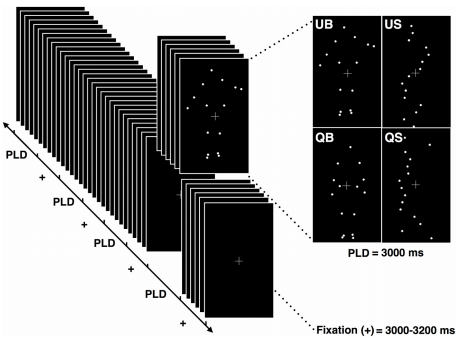
\includegraphics[width=8cm]{figvargas.png}
\caption{Schematics showing the whole experimental sequence split into blocks with visual stimulus (PLD) and rest state (+). Each condition (QB,QS,UB,US) is chosen at random. Image from \cite{vargas17}.}
\end{figure}

From the 256 runs completed by the individual, 64 were in each condition, in random order. However, the subject unfortunately blinked in most runs. Blinking produces a large disruption across \emph{all} channels, which might be tricky to remove without impairing the confidence on the results. This is why for this initial sample we have selected only those runs without blinks - only 17 in total. 

The EEG signal was captured with a 128-electrode cap (HydrocCel Geodesic Sensor Net). The original data contained the signals from each electrode referenced to the vertex (VREF on figure \ref{figtouca}, often also called CZ). The original sampling frequency was 500Hz. However, some first-level pre-processing had been done already in order to remove ambient and experimental noise. It included applying a 60Hz filter to remove line noise and downsampling to 100Hz.

\begin{figure}[H]\label{figtouca}
\centering
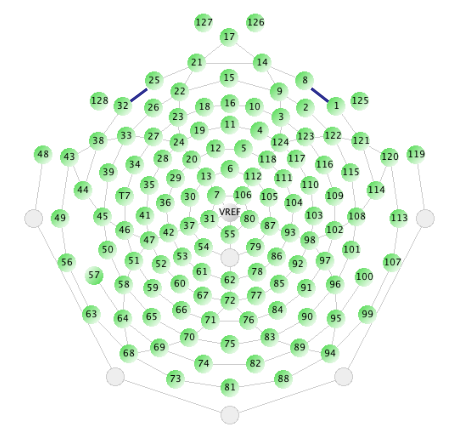
\includegraphics[width=8cm]{128cap.png}
\caption{Schematics of the electrode positions. Image from the device manual.}
\end{figure}

\newpage
\subsection{Selected datasets}

These are the runs without blinks from subject 13.

\begin{table}[H]
\begin{tabular}{lll}
Selected runs name & Original name   & Stimulus type \\
1 & 121 & QS\\
2 & 131 & QB\\
3 & 221 & HS\\
4 & 227 & HB\\
5 & 230 & QS\\
6 & 307 & HB\\
7 & 311 & HB\\
8 & 424 & HB\\
9 & 431 & QB\\
10& 504 & QS\\
11& 626 & QS\\
12& 704 & HB\\
13& 710 & QS\\
14& 712 & QS\\
15& 715 & HS\\
16& 729 & HB\\
17& 804 & HS
\end{tabular}
\end{table}

\section{Pre-processing}

We applied the following additional pre-processing steps to the selected runs:

\begin{itemize}

\item A Butterworth highpass filter at 1Hz, in order to cut drifts and other low period contributions (e.g. heartbeat effects)
\item A Butterworth lowpass filter at 50Hz, in order to be sure that ambient noise and electrical static effects are removed
\item Re-referencing. The original reference at the scalp vertex is not ideal due to a slight variation in positioning from experiment to experiment and the observation a full brain long-term oscillations actually resulting from oscillations on the reference. We re-referenced to the average signal from all electrodes, as standard, using EEGLab.
\end{itemize}

\subsection{Comments}
\begin{itemize}
\item Also using EEGLab, we have used Independent Component Analysis (ICA) to identify blink-related or mechanical motion components that went unchecked, however these where not found on the 17 selected runs, which is as desired. 

\item Future work: We are considering ways of removing outlier electrode signals. Whereas some groups prefer to look for different statistics, others recommend deletion by visual inspection. We are favourable to check the variance of each channel and delete the outliers given a certain threshold, which is yet to be defined. In principle, this favours automation, which will be essential as we add other runs and subjects.
\end{itemize}



\section{First analysis on the individual datasets}

We next performed separately the correlation analysis between the signal from one electrode with the signal from all others in the scalp for each selected condition. The resulting correlation coefficients and p-values are expressed in matrices given in supplementary file \hl{filename}. Alternatively, they can be expressed in 2-D or 3-D head plots such as figures \ref{fig:topoplot} and \ref{fig:headplot} below, which represents the result for the first selected dataset during stimulus (QS). In the case of the topographic 2D head plot, electrodes positioned on the laterals of the scalp or in front/back of the head are plotted as \textit{outside} the 2D head line. The case for how the signal from each electrode correlates with the others can be seen in Figs. \ref{fig:topomap1} and \ref{fig:topomap2}.

\begin{figure}[H]
    \centering
    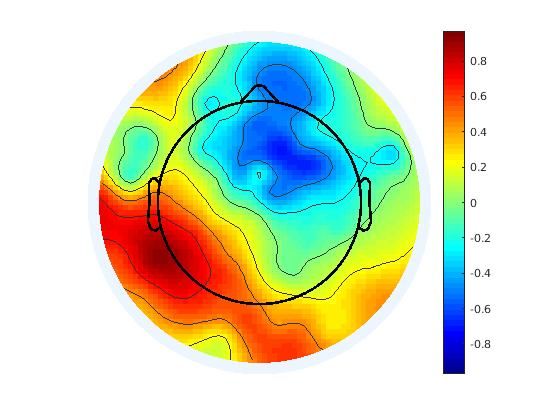
\includegraphics[width=10cm]{topoplot.jpg}
    \caption{2D head plot of the correlation coefficient of the signal at electrode 50 with the other brain areas during visual stimulus QS in the first selected block}
    \label{fig:topoplot}
\end{figure}

\begin{figure}[H]
    \centering
    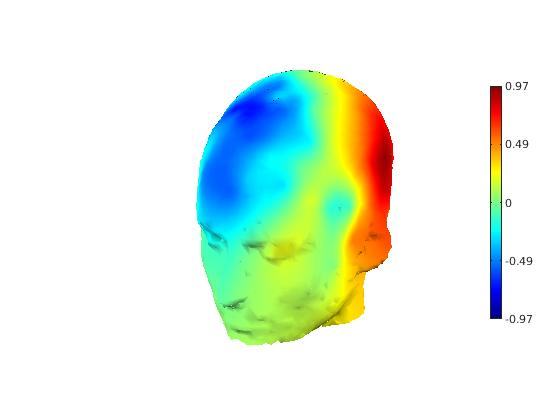
\includegraphics[width=10cm]{headplot.jpg}
    \caption{3D head plot of the correlation coefficient of the signal at electrode 50 with the other brain areas during visual stimulus QS in the first selected block}
    \label{fig:headplot}
\end{figure}

\begin{figure}[H]
    \centering
    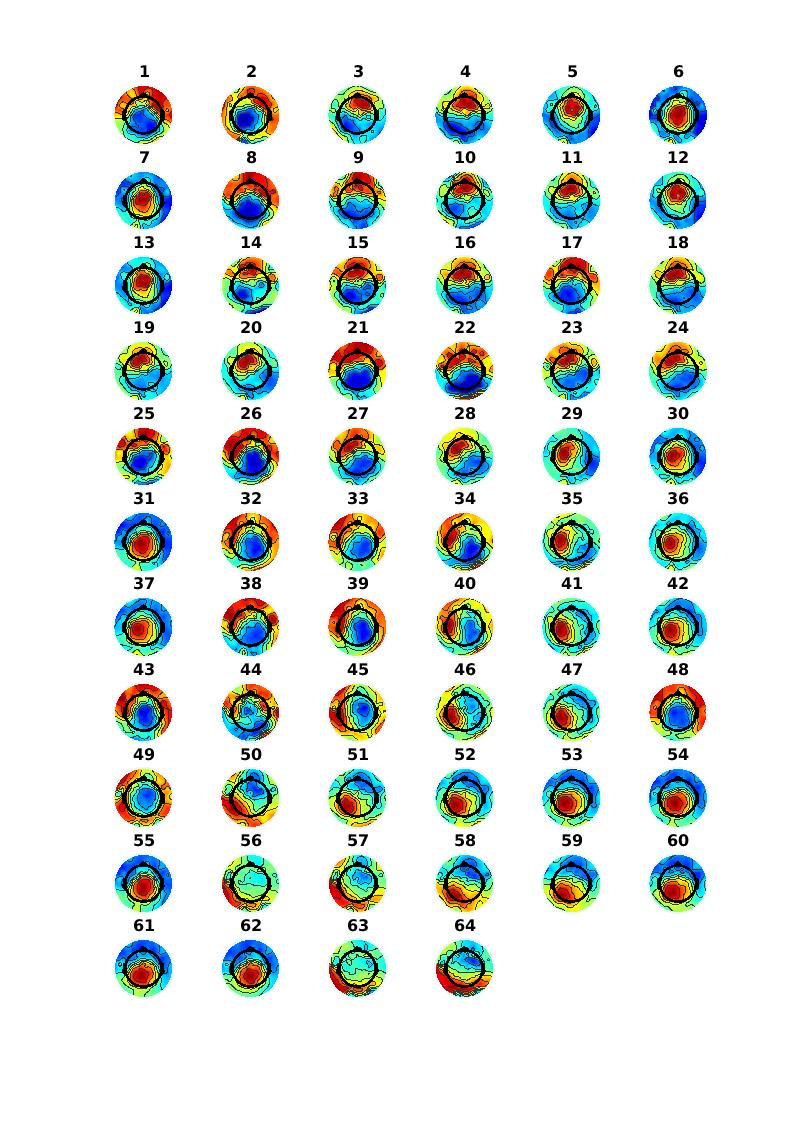
\includegraphics[width=16cm]{map1.jpg}
    \caption{2D head plots of the correlation coefficient of the signal at each electrode (each plot) with the other brain areas during visual stimulus QS in the first selected block}
    \label{fig:topomap1}
\end{figure}

\begin{figure}
    \centering
    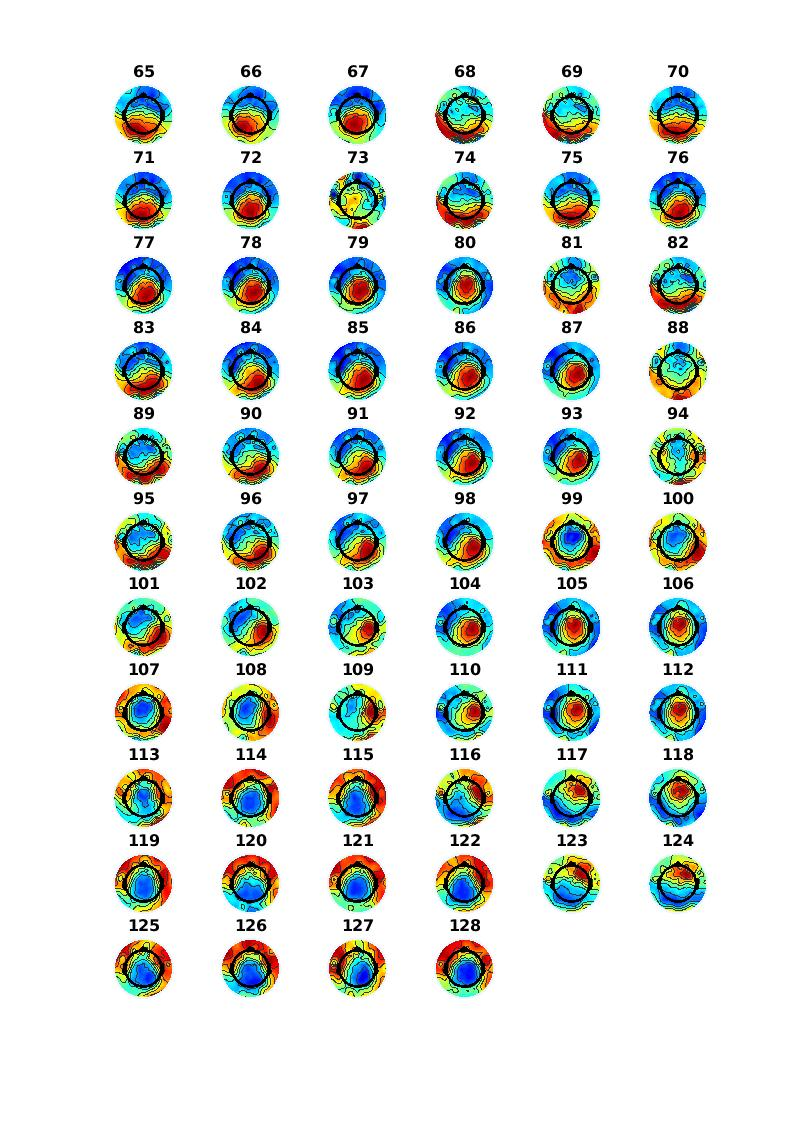
\includegraphics[width=16cm]{map2.jpg}
    \caption{Continuation of figure \ref{fig:topomap1}, \textit{i.e.}, 2D head plots of the correlation coefficient of the signal at each electrode (each plot) with the other brain areas during visual stimulus QS in the first selected block}
    \label{fig:topomap2}
\end{figure}

\newpage

The dipole effect observed above does not truly reflect the nature of brain functional links. One of the caveats in using correlation function is that the effect of time is not considered: neurons more distantly connected are not expected to have an immediate effect but a delayed one. The observation at a fixed time $t=t'$ is likely to be majored by the global equilibrium of charge. However, the delay effect could be considered by computing the cross-correlation \textit{function}, and selecting the value at its peak. In addition we obtain from the method the lag to which this maximum is obtained (Fig. \ref{fig:xcorr}). The topographic plot (Fig. \ref{fig:topoplot2}) immediately reduces the dipole effect. Also, the information about the lags allows the quick identification of the spurious correlations. The result for electrode 50 in 3D is displayed in Fig. \ref{fig:headplot2}, and the 2D results for the other electrodes is given in Figs. \ref{fig:topomapfun1} and \ref{fig:topomapfun2}.

\vspace{3cm}

\begin{figure}[H]
    \centering
    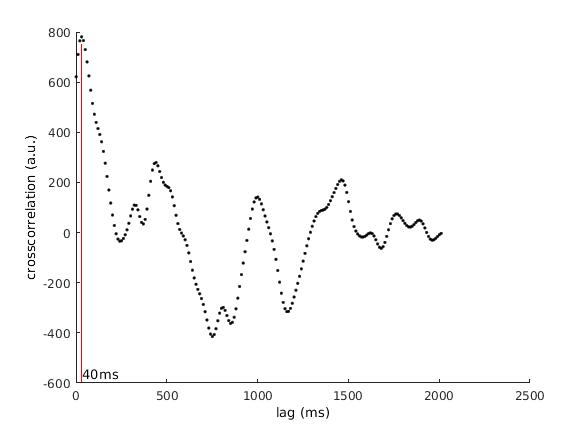
\includegraphics[width=10cm]{correlation.jpg}
    \caption{Cross-correlation function of the signal from node 50 and signal from node 70 for 200ms of the stimulus QS in the first selected dataset. Observe the maximum occurring at the lag 40ms.}
    \label{fig:xcorr}
\end{figure}

\newpage

\begin{figure}[H]
    \centering
    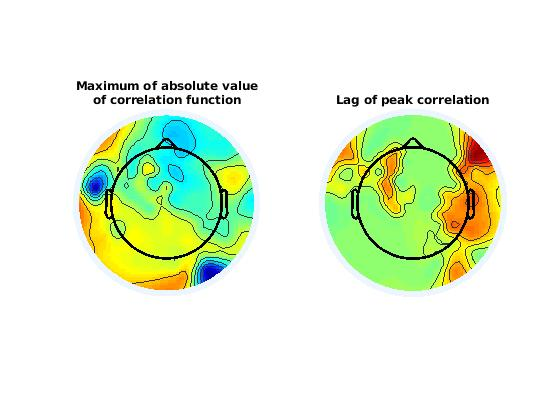
\includegraphics[width=13cm]{topoplot2.jpg}
    \caption{2D head plot of the maximum correlation function (left) and respective lag (right) for the signal at electrode 50 with the other brain areas during visual stimulus QS in the first selected block. For high lag areas (yellow and red in the right plot) the correlation on the left plot is likely spurious}
    \label{fig:topoplot2}
\end{figure}

\begin{figure}[H]
    \centering
    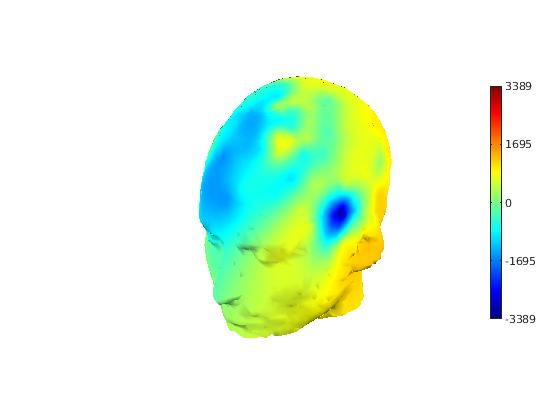
\includegraphics[width=10cm]{headplot2.jpg}
    \caption{3D head plot of the maximum correlation function of the signal at electrode 50 with the other brain areas during visual stimulus QS in the first selected block}
    \label{fig:headplot2}
\end{figure}


\begin{figure}[H]
    \centering
    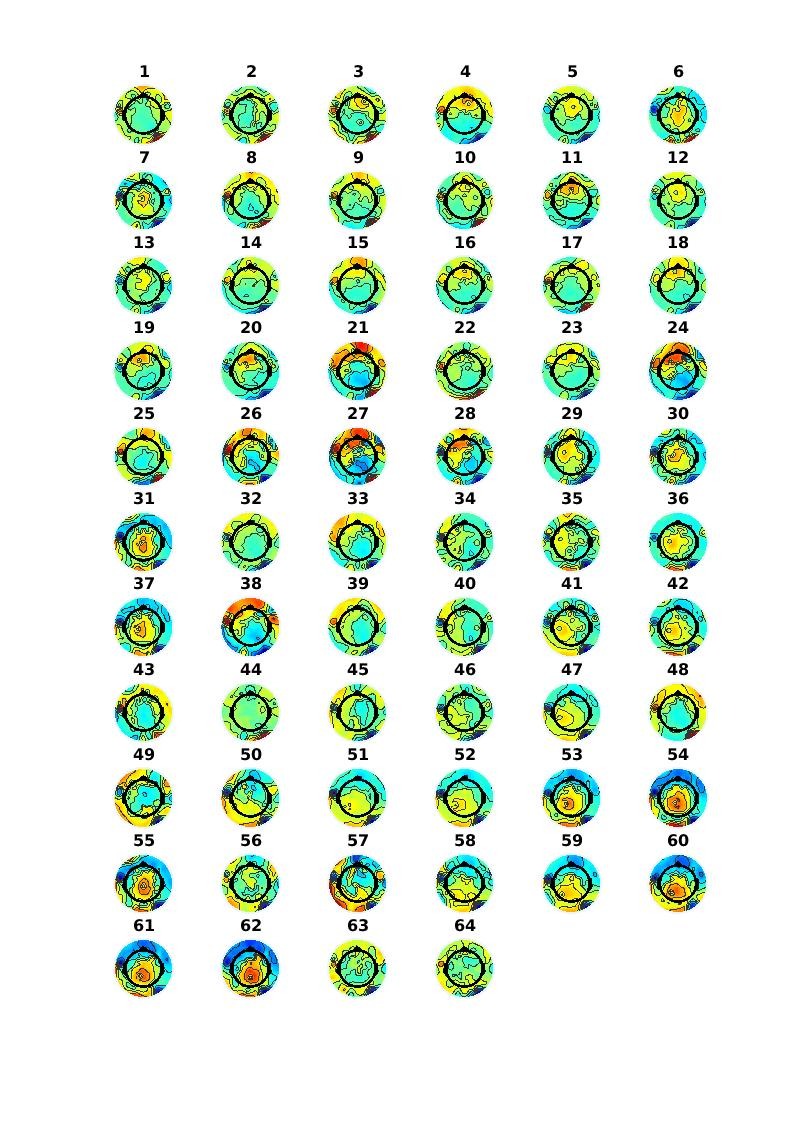
\includegraphics[width=15cm]{topomapfun1.jpg}
    \caption{2D head plots of the maximum of correlation function of the signal at each electrode (each plot) with the other brain areas during visual stimulus QS in the first selected block}
    \label{fig:topomapfun1}
\end{figure}

\begin{figure}
    \centering
    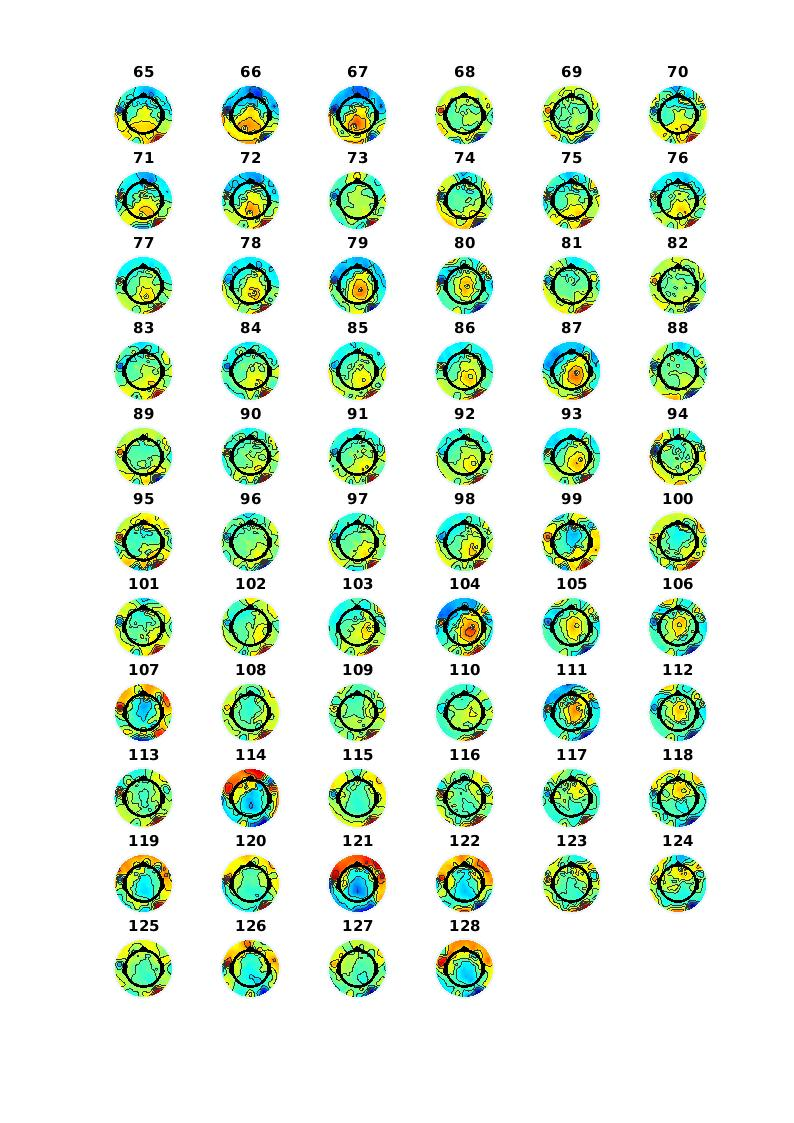
\includegraphics[width=15cm]{topomapfun2.jpg}
    \caption{Continuation of figure \ref{fig:topomapfun1}, \textit{i.e.}, 2D head plots of the maximum of correlation function of the signal at each electrode (each plot) with the other brain areas during visual stimulus QS in the first selected block}
    \label{fig:topomapfun2}
\end{figure}


\section{Average correlation results for subject 13}

The second stage was to perform the analysis of the average for each stimulus type for subject 13. (The third stage will be to average over the individuals, so to have a group result of the response to each kind of stimulus). Figures \ref{fig:avgtopoplot} and \ref{fig:avgheadplot} show the result of the average correlation from signal at electrode 50 to other brain areas during stimulus QS. Figures \ref{avgmap1.jpg} and \ref{avgmap2.jpg} show the results for the other electrodes. As expected, the correlation is typically higher around the electrode position, but, occasionally, correlated areas form in other regions. 


\begin{figure}[H]
    \centering
    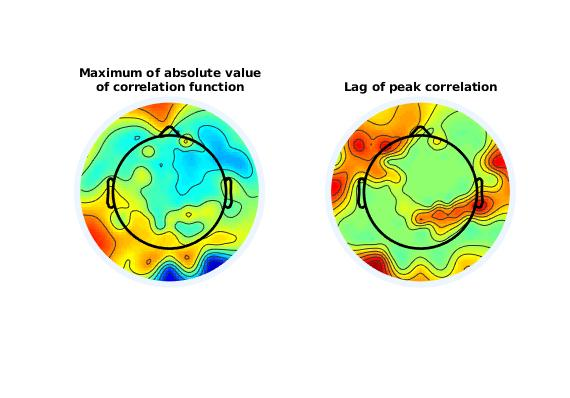
\includegraphics[width=10cm]{avgtopoplot.jpg}
    \caption{2D head plot of the maximum correlation function (left) and respective lag (right) for the signal at electrode 50 with the other brain areas during visual stimulus QS. This time the result is the average over 6 trials for subject 13. For high lag areas (yellow and red in the right plot) the correlation on the left plot is likely spurious}
    \label{fig:avgtopoplot}
\end{figure}

\begin{figure}[H]
    \centering
    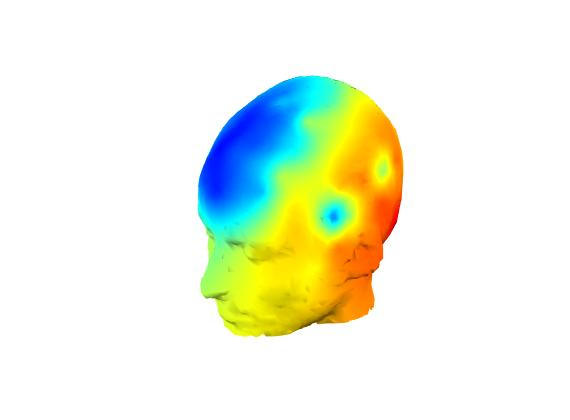
\includegraphics[width=10cm]{avgheadplot.jpg}
    \caption{3D head plot of the maximum correlation function for the signal at electrode 50 with the other brain areas during visual stimulus QS. This time the result is the average over 6 trials for subject 13. For high lag areas (yellow and red in the right plot) the correlation on the left plot is likely spurious}
    \label{fig:avgheadplot}
\end{figure}

\begin{figure}[H]
    \centering
    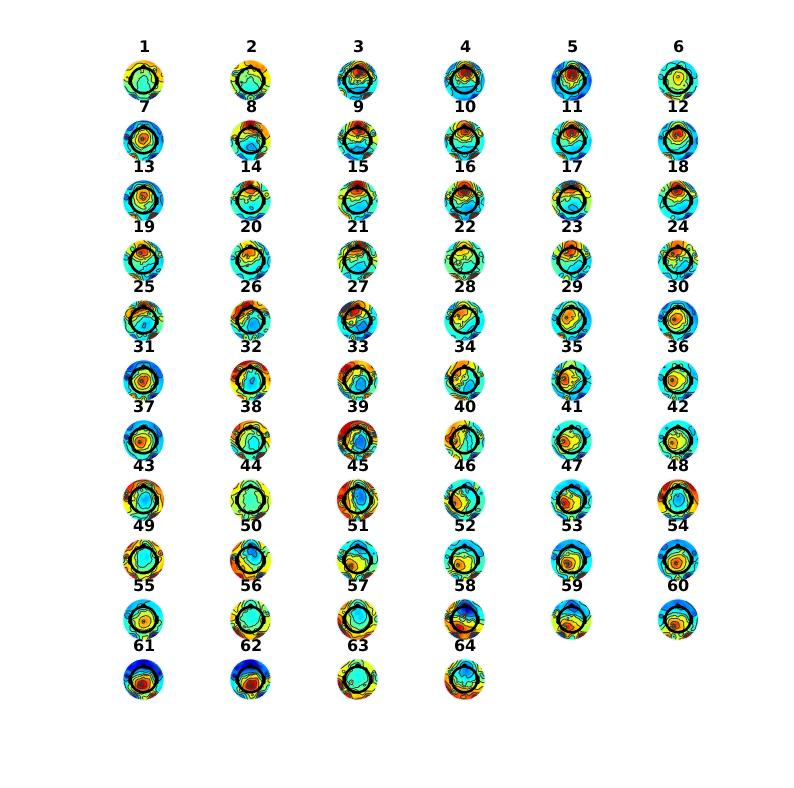
\includegraphics[width=16cm]{avgmap1.jpg}
    \caption{2D head plots of the maximum of correlation function of the signal at each electrode (each plot) with the other brain areas during visual stimulus QS. Average over 6 trials of subject 13.}
    \label{fig:avgmap1}
\end{figure}

\begin{figure}
    \centering
    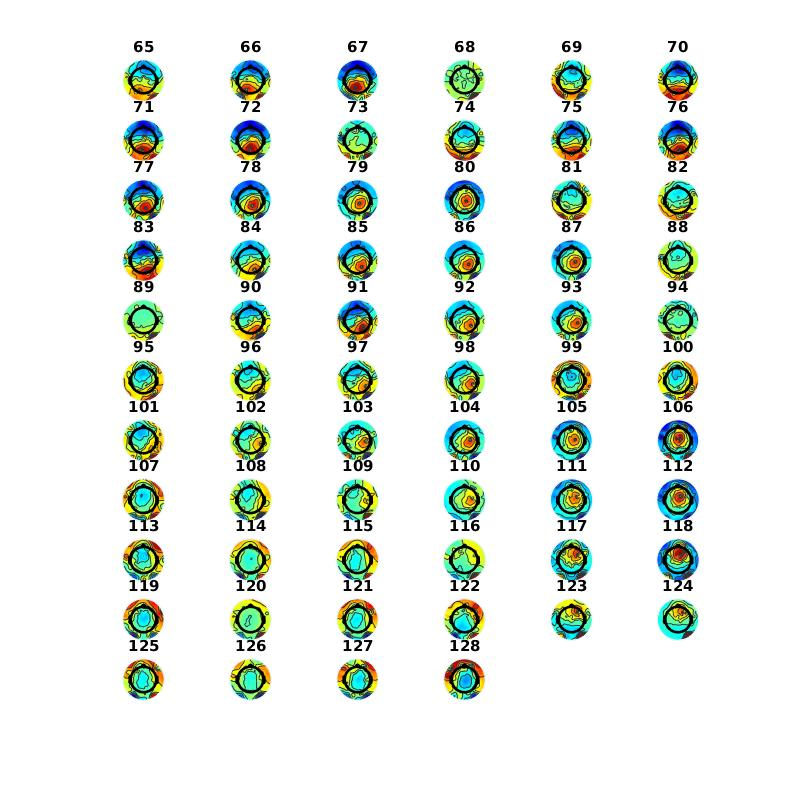
\includegraphics[width=16cm]{avgmap2.jpg}
    \caption{Continuation of figure \ref{fig:topomapfun1}, \textit{i.e.}, 2D head plots of the maximum of correlation function of the signal at each electrode (each plot) with the other brain areas during visual stimulus QS. Average over 6 trials of subject 13.}
    \label{fig:avgmap2}
\end{figure}

\newpage

In this procedure, it is not yet clear what is the effect from the brain regular activity, and what is the effect from the stimulus. So, in the next subsections we will subtract the correlation from the stimulus from the correlation during rest state. In addition, we will define as 0 the correlation for which the lag of the peak is above 50ms, as any value obtained is likely spurious. Results, we will see, are much clearer with respect to the identification of the brain areas most associated to each stimulus, by the definition of sharper regions with high net correlation.

\subsection{Net effect of QB stimulus}

\begin{figure}[H]
    \centering
    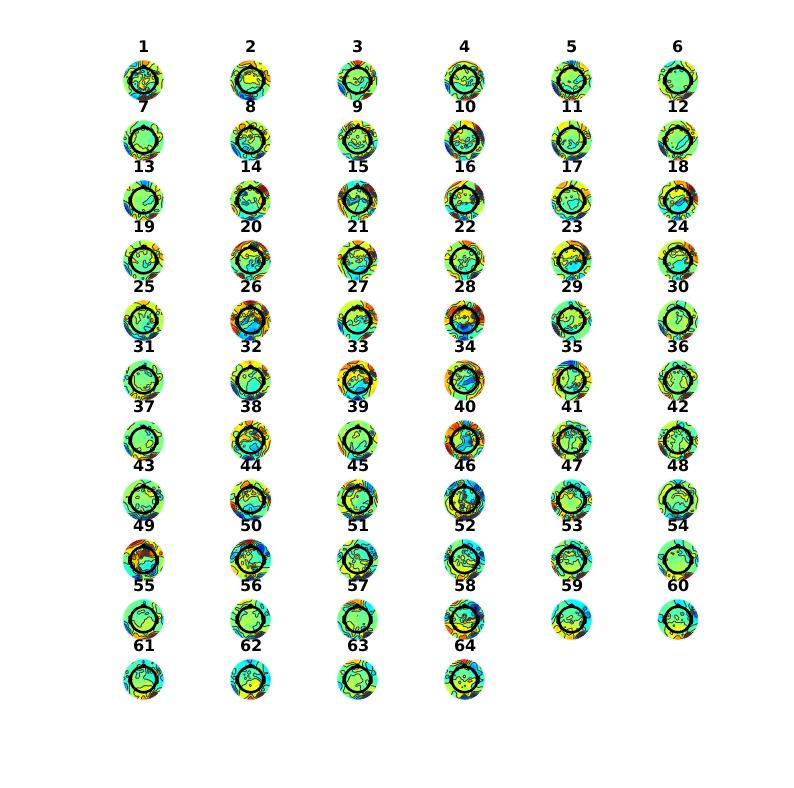
\includegraphics[width=16cm]{QB1.jpg}
    \caption{2D head plots of the net effect of stimulus QB for the signal at each electrode to other brain areas. It is computed as the difference of the maximum of correlation function of the signal during stimulus and during the rest state. Average over 2 trials of subject 13.}
    \label{fig:qb1}
\end{figure}

\begin{figure}
    \centering
    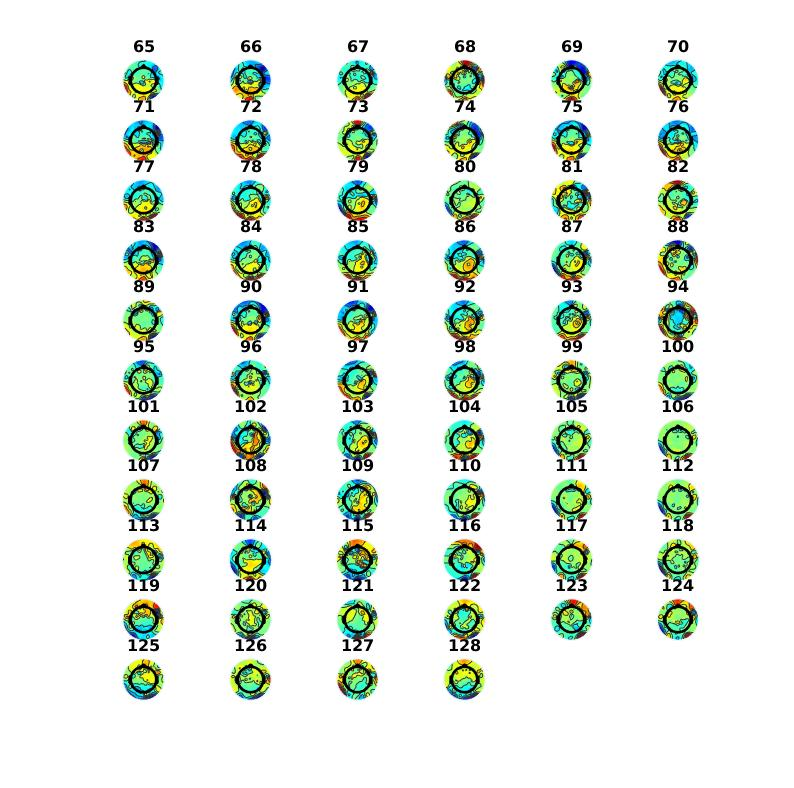
\includegraphics[width=16cm]{QB2.jpg}
    \caption{Continuation of figure \ref{fig:topomapfun1}, \textit{i.e.}, 2D head plots of the net effect of stimulus QB for the signal at each electrode to other brain areas. It is computed as the difference of the maximum of correlation function of the signal during stimulus and during the rest state. Average over 2 trials of subject 13.}
    \label{fig:qb2}
\end{figure}

\subsection{Net effect of QS stimulus}

\begin{figure}[H]
    \centering
    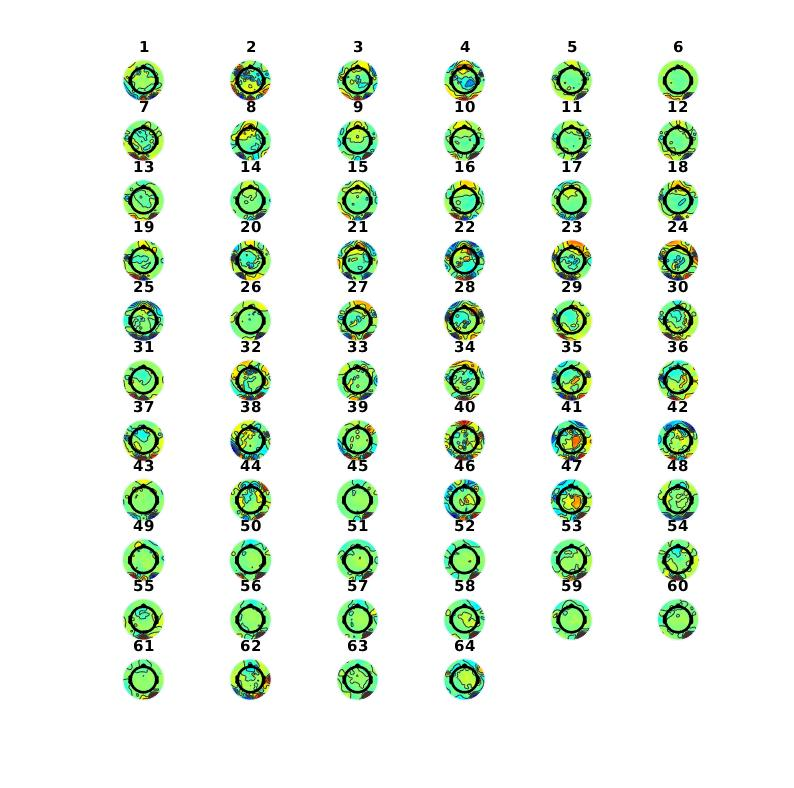
\includegraphics[width=16cm]{QS1.jpg}
    \caption{2D head plots of the net effect of stimulus QS for the signal at each electrode to other brain areas. It is computed as the difference of the maximum of correlation function of the signal during stimulus and during the rest state. Average over 2 trials of subject 13.}
    \label{fig:qs1}
\end{figure}

\begin{figure}
    \centering
    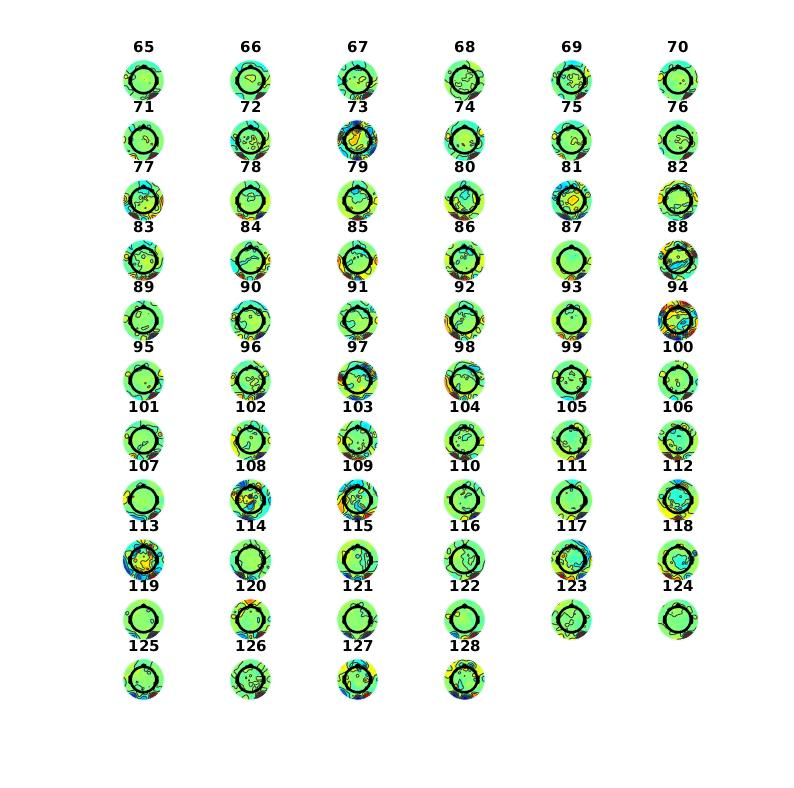
\includegraphics[width=16cm]{QS2.jpg}
    \caption{Continuation of figure \ref{fig:topomapfun1}, \textit{i.e.}, 2D head plots of the net effect of stimulus QS for the signal at each electrode to other brain areas. It is computed as the difference of the maximum of correlation function of the signal during stimulus and during the rest state. Average over 2 trials of subject 13.}
    \label{fig:qs2}
\end{figure}

\subsection{Net effect of HB stimulus}

\begin{figure}[H]
    \centering
    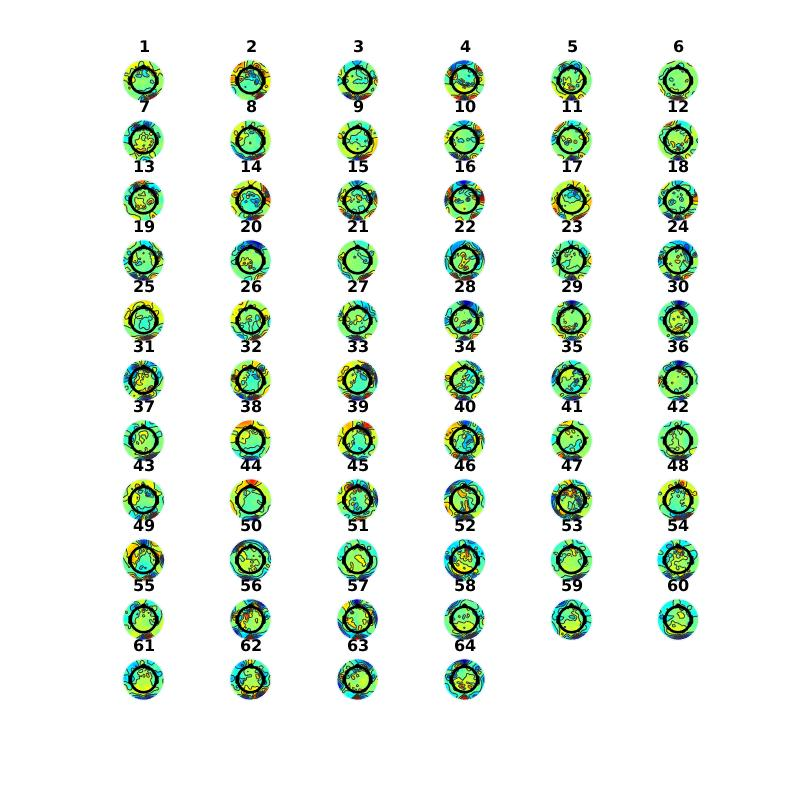
\includegraphics[width=16cm]{HB1.jpg}
    \caption{2D head plots of the net effect of stimulus HB for the signal at each electrode to other brain areas. It is computed as the difference of the maximum of correlation function of the signal during stimulus and during the rest state. Average over 6 trials of subject 13.}
    \label{fig:hb1}
\end{figure}

\begin{figure}
    \centering
    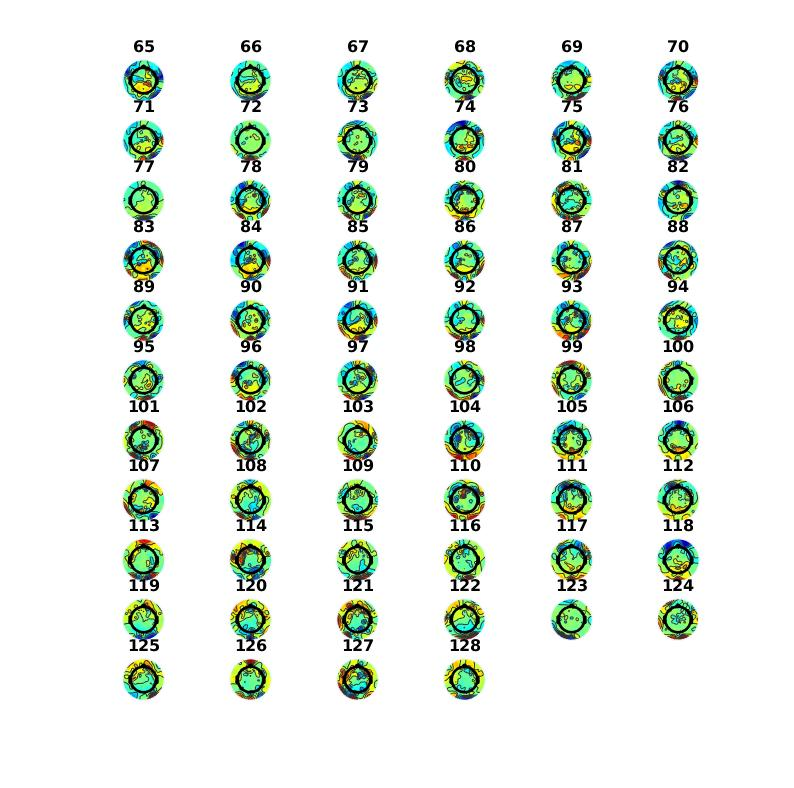
\includegraphics[width=16cm]{HB2.jpg}
    \caption{Continuation of figure \ref{fig:topomapfun1}, \textit{i.e.}, 2D head plots of the net effect of stimulus HB for the signal at each electrode to other brain areas. It is computed as the difference of the maximum of correlation function of the signal during stimulus and during the rest state. Average over 6 trials of subject 13.}
    \label{fig:hb2}
\end{figure}

\subsection{Net effect of HS stimulus}

\begin{figure}[H]
    \centering
    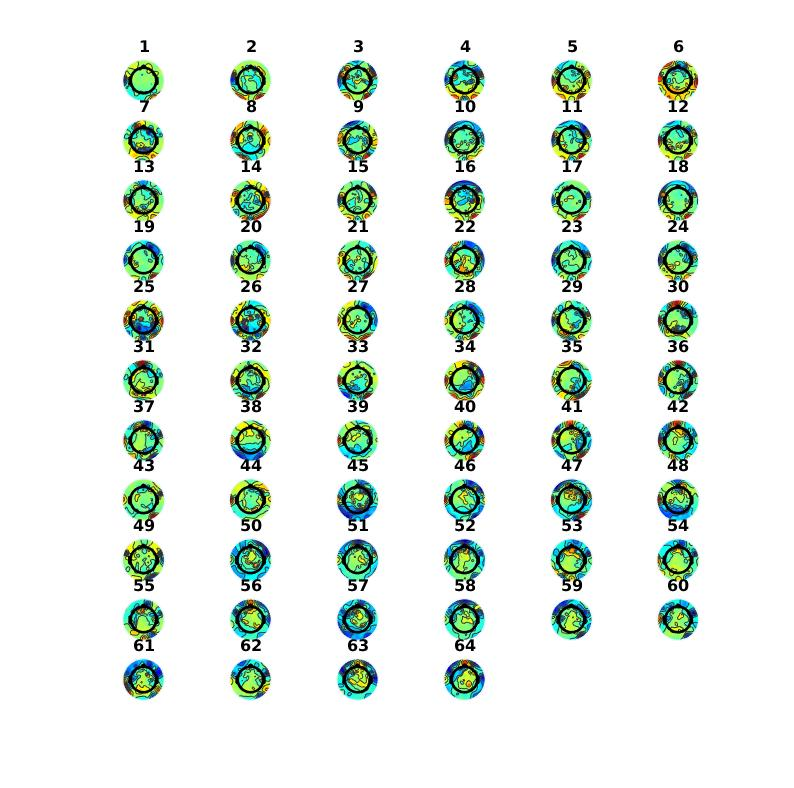
\includegraphics[width=16cm]{HS1.jpg}
    \caption{2D head plots of the net effect of stimulus HS for the signal at each electrode to other brain areas. It is computed as the difference of the maximum of correlation function of the signal during stimulus and during the rest state. Average over 3 trials of subject 13.}
    \label{fig:hs1}
\end{figure}

\begin{figure}
    \centering
    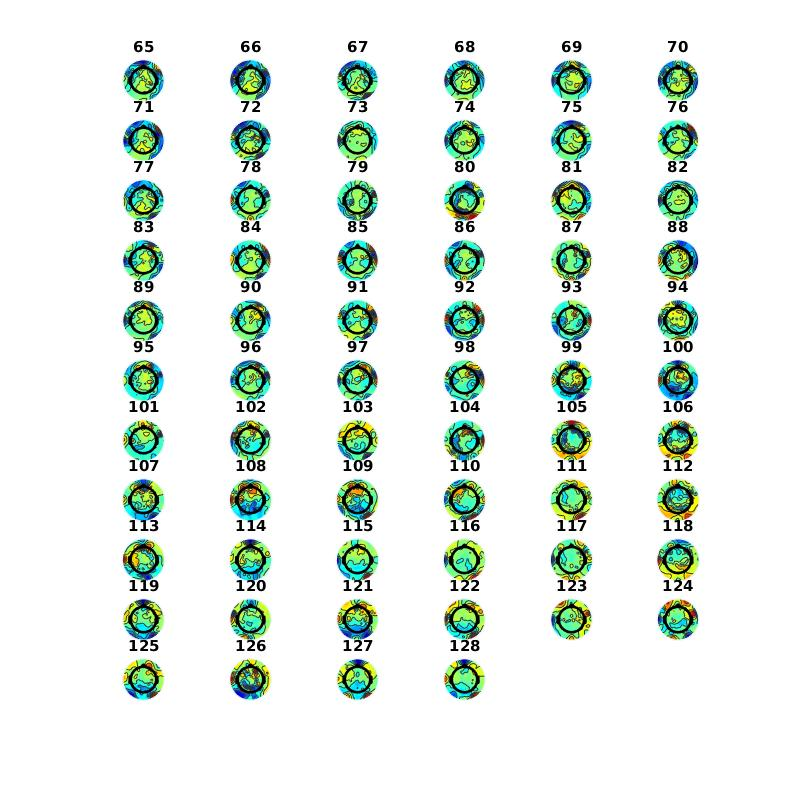
\includegraphics[width=16cm]{HS2.jpg}
    \caption{Continuation of figure \ref{fig:topomapfun1}, \textit{i.e.}, 2D head plots of the net effect of stimulus HS for the signal at each electrode to other brain areas. It is computed as the difference of the maximum of correlation function of the signal during stimulus and during the rest state. Average over 3 trials of subject 13.}
    \label{fig:hs2}
\end{figure}

\newpage
\section{Analysis of dynamical connectivity}

It is an analysis of how the brain network changes \emph{during} the experiment. This part was proposed together with Rodrigo Rocha (NeuroMat postdoc, FFCLRP-USP). Three options are considered:

\begin{itemize}
    \item Over time intervals (five are initially proposed: the rest state, the beginning of the stimulus, two at the stimulus main range, at the end of the stimulus)
    \item Over sliding windows
    \item Using principle of dynamic functional connectivity, which provides the connectivity matrix at each time-series point
\end{itemize}

Discussions are under way. One of the key aspects we want to investigate is the transient effect from the rest state to the stimulus. The second question is how this initial reaction later on evolves from learning to a short visual memory response.

In addition, we consider to extend the analysis for the effect observed at each frequency band, to check different behaviours between brain alpha rhythm and gamma oscillations, for example. (Reminding that gamma oscillations are mostly associated with cognitive processes). 

\section{Non-linear time-series analysis and information theory}

After cleaning of blinks in the remaining trials from subject 13 we may have sufficient data to perform analysis of Lyapunov exponents, entropy-complexity mapping, mutual information, causal mutual information and transfer entropy in the system. 

These methods will: (1) help distinguish the regime of the system (linear, chaotic, noisy, etc), (2) identify the shared information and the transfer of information between brain regions, (3) support inference of functional links between brain areas that could be previously hidden when adopting the cross-correlation strategy. 

With the currently selected dataset, though, it is impossible to perform such analysis reliably, once we have only 17 short trials.

\bibliographystyle{unsrtnat}
\bibliography{sample}

\end{document}